% ============================================================================
%  Schelling-Point Reputation Communities
%  A Decentralized Guarantee and Arbitration Layer for Agent-to-Agent Commerce
%
%  Main file. Compile: pdflatex main && bibtex main && pdflatex main && pdflatex main
%  Chapters: intro (1) / related-work (2) / ita-architecture (3) /
%            mech-design (4) / implementation (5) / conclusion (6)
% ============================================================================
\documentclass[11pt]{article}

\usepackage[margin=1in]{geometry}
\usepackage{amsmath,amssymb,amsfonts}
\usepackage{amsthm}
\usepackage{graphicx}
\usepackage{booktabs}
\usepackage{array}
\usepackage{enumitem}
\usepackage{hyperref}
\usepackage{xcolor}

\hypersetup{
  colorlinks=true, linkcolor=blue!60!black, citecolor=green!40!black,
  urlcolor=blue!60!black, pdfauthor={}, pdftitle={Schelling-Point Reputation Communities}
}

% ---------- theorem 环境（全局连续编号，供第 4/5 章复用） ----------
\newtheorem{theorem}{Theorem}[section]
\newtheorem{lemma}[theorem]{Lemma}
\newtheorem{proposition}[theorem]{Proposition}
\newtheorem{corollary}[theorem]{Corollary}
\newtheorem{definition}[theorem]{Definition}
\newtheorem{remark}[theorem]{Remark}
\newtheorem{example}[theorem]{Example}

% ---------- 图形路径：仿真图统一指向 simulation/plots/ ----------
\graphicspath{{../simulation/plots/}}

\title{\textbf{Schelling-Point Reputation Communities: A Decentralized Guarantee and Arbitration Layer for Agent-to-Agent Commerce}}
\author{
  AgentTrust Protocol Team\\[2pt]
  \small \texttt{github.com/Fishman-free/multiagent}
}
\date{\today}

\begin{document}

\maketitle

\begin{abstract}
As large language models and tool-use capabilities mature, AI agents are evolving from
analytical tools into counterparties capable of autonomously negotiating, signing, transferring
funds, and settling. When agents hold funds and act as ``digital twins'' of humans, anonymous,
machine-to-machine commerce raises a new class of trust problems: how can agents establish mutual
trust, and how can malicious agents be held accountable after misbehavior? We present a
decentralized guarantee and arbitration layer for agent-to-agent commerce built on four production
Solidity contracts --- an agent registry, a guaranteed escrow, a staked-voting arbitration
mechanism, and an on-chain reputation hub --- and formalize its core mechanism, the
\emph{Schelling-point reputation community}: a set of staked voters who adjudicate trade disputes,
whose verdicts drive the release of escrowed funds and the update of on-chain reputation, and whose
reputation scores in turn price the guarantees that make future trades safe. We prove that honest
voting is an incentive-compatible equilibrium under a two-thirds supermajority rule (an attack by a
minority of at most $35\%$ of voters is strategically harmless), that Sybil attacks are
unprofitable because adversarial voting power scales linearly in expenditure, and that the mechanism
conserves funds exactly. We instantiate the protocol in Solidity (38 tests), validate the game-theoretic
claims by Monte-Carlo simulation built on \textsf{mesa}, and discuss deployment to a public testnet.
\end{abstract}

{\small
\noindent\textbf{Keywords:} AI agents; blockchain; decentralized arbitration; staked voting;
Schelling points; reputation; guaranteed escrow; agentic commerce.
}

% ============================================================================
%  Chapter 1: Introduction
% ============================================================================
\section{Introduction}
\label{sec:intro}

\paragraph{Background: from analysis tool to digital-twin counterparty.}
Large language models (LLMs) and tool-use capabilities have made AI agents able to plan
autonomously, call external tools, and execute multi-step tasks. The decisive shift is that an
agent is no longer merely a system that \emph{answers questions}; it can make economically
consequential commitments on behalf of its owner --- negotiating prices, signing terms, initiating
transfers, and settling smart contracts. When an agent holds funds and can complete payments, it
effectively constitutes a ``digital twin'' trading counterparty of its human owner.

This trend has given rise to agentic commerce and agent-to-agent (A2A) finance as research
categories \cite{a2a-finance, agent-rep}. Prior work observes that AI agents are transitioning from
analysis tools into counterparties, generating a demand for financial-grade infrastructure for
identity, authorization, payment, verification, reputation, and accountability. However,
widespread adoption amplifies three systemic risks: \emph{identity fraud} --- anyone can cheaply
mass-produce ``fake agents''; \emph{mutual-trust deficit} --- an anonymous counterparty cannot
tell whether the other side is trustworthy; and \emph{accountability vacuum} --- after an agent
misbehaves there is no clear path to attribute fault, present evidence, and impose sanctions.

\paragraph{Problem statement.}
We focus on three interconnected questions:

\begin{itemize}[leftmargin=2em,itemsep=1pt]
  \item \textbf{Q1 (Trust).} When agents transact on behalf of humans, how can mutual trust be
  established so that ``scammer agents'' do not infiltrate?
  \item \textbf{Q2 (Accountability).} When a scammer agent commits fraud, how are fault, evidence,
  and sanctions determined?
  \item \textbf{Q3 (Incentives).} Which economic and governance mechanisms make the trust
  infrastructure self-sustaining and scalable?
\end{itemize}

These questions restate the classic trust problem in a machine-to-machine, anonymity-by-default
setting: trust must come not from knowing a counterpart's history but from a verifiable, auditable,
and traceable technical infrastructure.

\paragraph{Our approach: a Schelling-point reputation community.}
We design and implement a decentralized guarantee and arbitration layer for agent-to-agent
commerce. The system is organized along the identity--trust--accountability (ITA) architecture
(Section~\ref{sec:ita}): a registry issues ERC-721 agent identities bound to real principals; a
guaranteed escrow escrows trade funds against guarantor stakes; disputes are adjudicated by a
community of staked voters whose majority --- by a Schelling-point argument --- is incentivized to
vote truthfully; and a reputation hub records outcomes on-chain and prices future guarantees. The
central novelty is the \emph{closed loop}: verdicts update reputation, reputation prices the
guarantee, and the guarantee determines whether low-reputation agents can transact at all
(Section~\ref{sec:pricing}).

The mechanism is instantiated by four production Solidity contracts (Section~\ref{sec:contracts})
with 38 passing tests, and its game-theoretic claims are validated by Monte-Carlo simulation
(Section~\ref{sec:eval}).

\paragraph{Contributions.}
\begin{itemize}[leftmargin=2em,itemsep=1pt]
  \item \textbf{A closed-loop mechanism} connecting adjudication, guarantees, and reputation --- the
  first, to our knowledge, to tie all three into one on-chain cycle (Sections~\ref{sec:mech},
  \ref{sec:pricing}).
  \item \textbf{A formal game-theoretic analysis} of the staked-voting mechanism: honest voting is
  an incentive-compatible equilibrium under a two-thirds supermajority rule; a coordinated
  malicious minority of at most $35\%$ of voters is strategically harmless; Sybil attacks are
  unprofitable because adversarial voting power scales linearly in expenditure; and the mechanism
  conserves funds exactly (Section~\ref{sec:analysis}).
  \item \textbf{A production implementation} --- four verified-style Solidity contracts, 38 tests,
  an end-to-end demo flow, and Docker one-command bootstrapping --- together with a
  \textsf{mesa}-based simulation that empirically validates the theory (Section~\ref{sec:impl}).
  \item \textbf{An honest evaluation} of the MVP's limitations (free-abstention refunds, integer
  dust, threshold approximation) and the deployment path to a public testnet
  (Sections~\ref{sec:eval}, \ref{sec:deploy}).
\end{itemize}

\paragraph{Organization.}
Section~\ref{sec:related-work} surveys related work. Section~\ref{sec:ita} presents the ITA
architecture and its mapping to the four contracts. Section~\ref{sec:mech} formalizes the mechanism
and proves its incentive properties. Section~\ref{sec:impl} describes the implementation and its
empirical evaluation. Section~\ref{sec:conclusion} concludes.

% ============================================================================
%  Chapter 2: Related Work
% ============================================================================
\section{Related Work}
\label{sec:related-work}

\subsection{Decentralized identity and verifiable credentials}
The W3C has standardized Decentralized Identifiers (DIDs) \cite{w3c-did} and Verifiable
Credentials (VCs) \cite{w3c-vc} as mutually independent, composable primitives: a DID is a
URI that resolves to a DID document carrying control and verification methods, and a VC is a
cryptographically verifiable data model for claims such as qualifications, authorization, and
reputation. Implementation layers such as ION \cite{ion} anchor DID operations on Bitcoin without
a new token. These standards provide the skeleton for issuing identities to agents, but they do not
by themselves determine how identities are trusted in commerce, how disputes are adjudicated, or
how reputation is priced --- the concerns of this paper.

\subsection{Soulbound tokens and bound NFTs}
Soulbound tokens (EIP-5192 \cite{eip-5192}) and account-bound NFTs (EIP-4973 \cite{eip-4973})
generalize non-transferability, letting an address hold verifiable, non-tradeable attestations of
membership, achievement, or commitment. In our architecture the agent identity (an ERC-721 in
\textsf{AgentRegistry}) is bound to a real principal at registration and cannot be detached from the
responsibility it carries --- the accountability analogue of the soulbound idea.

\subsection{Autonomous accounts and payments}
Account abstraction (ERC-4337 \cite{eip-4337}) separates the signing key from the account logic,
enabling agents to sponsor gas, batch operations, and authorize delegated execution. The
agent-to-agent finance literature \cite{a2a-finance} surveys blockchain payment and trust
infrastructure for autonomous agents. Our work assumes such an account layer as the substrate and
focuses on the higher-level question of how two accounts that have never met reach trust: guarantee,
adjudicate, and build reputation.

\subsection{On-chain reputation and attestation}
The Ethereum Attestation Service (EAS) \cite{eas} provides a general on-chain attestation
registry. AgentReputation \cite{agent-rep} proposes a decentralized reputation framework for
agentic AI. Recent datasets of blockchain-registered AI agents \cite{agent-dataset} indicate early
adoption of agent identity standards. These works establish that reputation \emph{can} be recorded
on-chain, but leave open who is authorized to write, how truthful attestations are incentivized, and
how reputation is priced into risk. Our reputation hub (Section~\ref{sec:contracts}) closes the
write-incentive gap by restricting writers to audited escrow/voting contracts (no self-rating) and
by coupling scores to guarantee pricing.

\subsection{Decentralized arbitration and guarantees}
Decentralized dispute resolution has been explored by Kleros \cite{kleros} (a jury selected from a
set of paid, random jurors), Aragon Court \cite{aragon} (aragon.org/dish), and UMA's optimistic
oracle \cite{uma} (price oracle with a challenge period). Kleros and Aragon Court select jurors by
\emph{lottery} and reward coherent majorities; UMA incentivizes truthful price reporting through
disputes and forfeits. These mechanisms share the Schelling-point insight --- that truthful
majorities are self-enforcing --- but none of them \emph{closes the loop} with reputation and
guarantee pricing: a Kleros verdict is final and does not update a merchant's future cost of doing
business. On the insurance side, Nexus Mutual \cite{nexus-mutual} runs a mutual cover pool with a
claims-assessment community. Our contribution is to make the guarantee itself (escrow plus
guarantor stake) the stake that voters price, and to make every verdict feed a reputation score that
prices the next guarantee --- a three-way closed loop (Section~\ref{sec:pricing}).

\subsection{Trust research specific to agents}
Recent work on trustworthy LLM agents \cite{agent-networks, zero-trust, insured-agents} and on
binding agent identities \cite{binding-id} converge on the need for attestation, insurance, and
verifiable accountability. ERC-8004 (trustless agents) \cite{erc8004} sketches an interoperability
standard. We position this paper as the first to combine, end-to-end and with a formal
incentive analysis, (i) a registered identity, (ii) a guaranteed escrow, (iii) staked-voting
arbitration, and (iv) reputation-driven guarantee pricing in a single protocol whose contracts and
empirical validation are public.

% ============================================================================
%  Chapter 3: The Identity--Trust--Accountability (ITA) Architecture
% ============================================================================
\section{The ITA Architecture}
\label{sec:ita}

This section describes \emph{what} the protocol records and \emph{how} it holds agents
accountable. The incentive layer that explains \emph{why} rational agents behave honestly is the
subject of Section~\ref{sec:mech}; the concrete contract implementation is
Section~\ref{sec:impl}.

\subsection{Design goals and threat model}
We model three classes of principals: agents $A_{i}$ (autonomous trading entities), certification
and guarantee providers $S$ (guarantors, premium setters), and adjudication/enforcement entities
$E$ (voters, settlement executors). The system is designed to uphold six trust properties:
\emph{identity authenticity} (every agent maps to a real principal), \emph{non-repudiation}
(commitments are provably attributable), \emph{traceability} (outcomes are auditable on-chain),
\emph{fairness} (disputes are decided by a verifiable, non-capturable process), \emph{incentive
compatibility} (honest behavior is a dominant/equilibrium strategy), and \emph{privacy
adjustability} (only necessary claims are exposed). It defends against four canonical attacks:
Sybil attacks (mass identity fabrication), reputation manipulation (self-rating or score farming),
delinquency-and-exit (misbehaving under one identity then abandoning it), and single-point-authority
abuse (a centralized credit adjudicator who simultaneously scores, revokes, and investigates).

\subsection{Layer 1 --- Identity}
The identity layer gives every agent a verifiable, principal-bound identity. Rather than
introducing new cryptographic primitives, it composes mature standards --- W3C DIDs/VCs, soulbound
tokens (EIP-5192/4973), account abstraction (ERC-4337), and proof-of-personhood --- into a
single on-chain registry. In our implementation, \textsf{AgentRegistry} mints an ERC-721 Agent ID
per registered agent, binds it to the caller (the responsible principal), and charges a
\emph{registration fee} to price identity creation and deter Sybils. The registry thereby answers
Q1's identity side: agents must ``obtain a license before trading.''

\subsection{Layer 2 --- Trust}
The trust layer records, qualifies, and prices evidence of good behavior. It stores reputation
profiles as on-chain attestations (the role of EAS in the standards survey), supports
contextualized multi-dimensional scoring, and authorizes delegated claims via VCs. In our
implementation, \textsf{ReputationHub} maintains per-agent multi-dimensional profiles
(completions, defaults, dispute wins/losses), restricts writers to audited escrow/voting contracts
(no self-rating), and exposes a scalar score that prices future guarantees
(Section~\ref{sec:pricing}).

\subsection{Layer 3 --- Accountability}
The accountability layer guarantees funds, adjudicates disputes, and sanctions misbehavior. It
combines guaranteed escrow (the role of Nexus Mutual-style insurance), decentralized arbitration
(the role of Kleros/UMA), and forfeiture/revocation. In our implementation,
\textsf{GuaranteeEscrow} escrows trade funds and holds guarantor stakes that are forfeited on
default, and \textsf{SchellingVoting} adjudicates disputes by staked community vote whose verdict
drives escrow release and reputation update.

\subsection{From centralized adjudicator to decentralized trust infrastructure}
A central design thesis, echoing the survey's analysis, is that a \emph{social-credit-style}
centralized adjudicator --- a single authority that scores, revokes, and investigates --- is a
single point of abuse, monopoly, privacy, and fairness failure. The ITA architecture therefore
shifts the design center from ``centralized credit adjudicator'' to ``operator and rule-setter of
decentralized trust infrastructure'': trust is maintained by verifiable code and multi-party
governance rather than by the subjective endorsement of a single authority. This motivates the
decision that dispute adjudication (the arbiter of what counts as good behavior) be decentralized
staked voting rather than a privileged contract owner --- the subject of Section~\ref{sec:mech}.

\section{Mechanism Design}
\label{sec:mech}

This section describes the inspected legacy mechanism and states only code-level or conditional
results. It deliberately does not assert that truthful voting is a strict Bayesian--Nash equilibrium,
that a $35\%$ coalition is harmless, that a Sybil attack is unprofitable, or that all funds are
exactly conserved. Those conclusions require assumptions or implementation properties absent from
the current evidence.

\subsection{Legacy mechanism}
\label{sec:mechanism}

For one disputed trade, let $m_B,m_S,m_\bot$ be the counts of BUYER, SELLER, and ABSTAIN votes.
Each address that votes deposits a fixed amount $v>0$. Define the effective-vote count
$T=m_B+m_S$; abstentions are excluded from both the threshold denominator and the quorum. The legacy
constants are
\[
  \kappa=\frac{6500}{10000}=0.65,\qquad \nu=3.
\]
Thus the mechanism does \emph{not} implement an exact two-thirds rule.

\begin{definition}[Legacy adjudication rule]
\label{def:rule}
If $T=0$, the case is void. Otherwise side $X\in\{B,S\}$ is selected when
$m_X\cdot10000\ge T\cdot6500$. A selected side produces an effective verdict only when
$T\ge\nu$; otherwise the case is void. Since $0.65>1/2$, both sides cannot satisfy the predicate
when $T>0$. In the inspected snapshot a void case triggers a full buyer-wins escrow settlement, while
all vote deposits are claimable as refunds.
\end{definition}

\begin{definition}[Legacy voter settlement]
\label{def:settlement}
In an effective case, each voter on the selected side receives
\[
  v+\left\lfloor\frac{v m_\ell}{m_w}\right\rfloor,
\]
where $m_w$ and $m_\ell$ are the winning and losing effective-vote counts. Losing voters receive
zero, and abstainers may reclaim $v$. In a void case every participant may reclaim $v$. Claims are
pull payments and therefore require each eligible address to transact successfully.
\end{definition}

\paragraph{Escrow linkage.}
The legacy escrow holds buyer amount $x$ and guarantor collateral
\[
  g=\left\lfloor\frac{x\gamma}{10^{18}}\right\rfloor.
\]
The premium $\pi$ is quoted but is not separately deposited.
The guard is $\pi\le x$, so \texttt{premium == amount} is accepted and makes the seller payment zero
on a seller-win or normal-release path; the code does not require a positive seller remainder. On a
full buyer win, the buyer is sent $x+g$. On a seller win or normal release, the seller is sent
$x-\pi$ and the guarantor is sent $g+\pi$. Partial buyer resolution sends the buyer
$\lfloor x\beta/10000\rfloor+g$ and the seller the remaining buyer principal.

\subsection{What the threshold does and does not imply}
\label{sec:analysis}

\begin{proposition}[Vote count required to select a side]
\label{prop:threshold}
Suppose $h$ effective votes oppose a coalition and all $c$ coalition votes support one side. That
side is selected by the legacy rule if and only if
\[
 c\ge\left\lceil\frac{13h}{7}\right\rceil.
\]
This is a deterministic statement about a fixed vote profile, not a profitability or truthfulness
claim.
\end{proposition}

\begin{proof}
The side is selected exactly when $c/(c+h)\ge0.65=13/20$. Rearranging gives $7c\ge13h$;
integrality gives the ceiling. The separate quorum condition must also hold.
\end{proof}

A coalition with at most $35\%$ of effective votes cannot by itself select its preferred side against
unanimous opposition. It is nevertheless not ``strategically harmless.'' If the opposing side has
less than $65\%$, neither side is selected and the case is void. Because void cases default to the
buyer, a coalition can change the economic outcome by inducing a void, particularly when it favors
the buyer. It can also bribe, split honest votes, exploit abstention, or benefit from signal errors.
The threshold provides a vote-count barrier, not general collusion resistance.

\subsection{Abstention and equilibrium status}
\label{sec:abstention}

The legacy payoff rule creates an unresolved participation problem. An abstainer receives net
monetary payoff zero after refund. A voter receives a positive bonus only if on an effective winning
side, loses $v$ if on an effective losing side, and receives zero net payoff if the case is void. If
$p_w$ and $p_\ell$ denote the probabilities that a contemplated vote is respectively winning and
losing, its expected net payoff is
\[
  p_w\left\lfloor\frac{v m_\ell}{m_w}\right\rfloor-p_\ell v,
\]
with the counts outcome-dependent. Voting beats abstention only when this expression is positive.
Signal accuracy $q>1/2$ alone does not establish that inequality, because the threshold, pivotality,
other strategies, correlated signals, and the possibility of a void all matter.

Consequently, the earlier strict-Bayesian--Nash statement and its proof are withdrawn. A future
analysis could establish a \emph{conditional} equilibrium under a fully specified prior, evidence
model, electorate-size distribution, participation reward, and strategy profile. The current score
contract records seller trade outcomes, not voter participation, so the proposed reputation loop
does not presently turn abstention into a repeated-game penalty. That integration remains future
work.

\subsection{Sybil cost is capital at risk, not proven loss}
\label{sec:sybil}

One address may vote once per case, but the inspected voting contract does not require the address to
hold a registered agent token. Creating additional voting addresses is therefore cheap. Each vote
must lock $v$ until settlement and claim, which creates a linear \emph{capital requirement}. It is
not an equal linear expenditure: a winning Sybil recovers principal and may earn a reward; a void-case
Sybil can reclaim principal; only a losing effective vote forfeits principal. Registration fees are
irrelevant to the legacy voting path unless a future release binds voters to registered identities.
Even with such a binding, whether a fee is a social cost, protocol revenue, refundable capital, or
attacker-controlled transfer depends on governance and ownership.

No ``Sybil attacks are unprofitable'' theorem follows from Proposition~\ref{prop:threshold}. Profit
also depends on the dispute value, side payments, opportunity cost and duration of locked capital,
probability of each outcome, gas, registration policy, and whether the attacker benefits from a void.
The prototype establishes only that each legacy vote requires contemporaneous stake.

\subsection{Conditional accounting}
\label{sec:accounting}

\begin{proposition}[Voting-pool claim accounting]
\label{prop:voting-accounting}
Assume a case reaches settlement; every eligible claimant claims exactly once; every transfer
succeeds; and no unrelated Ether is included. Then a void case makes claims totaling
$(m_B+m_S+m_\bot)v$. An effective case makes claims totaling
\[
 (m_B+m_S+m_\bot)v-\delta,
 \quad
 \delta=(v m_\ell)\bmod m_w,
 \quad 0\le\delta<m_w.
\]
The remainder $\delta$ remains in the contract unless a separate recovery mechanism exists.
\end{proposition}

\begin{proof}
The winning side claims
$m_wv+m_w\lfloor vm_\ell/m_w\rfloor=m_wv+vm_\ell-\delta$; abstainers claim
$m_\bot v$ and losers claim zero. The void expression follows because every participant is eligible
for principal. These are claim entitlements, not a liveness guarantee.
\end{proof}

\begin{proposition}[Escrow branch accounting]
\label{prop:escrow-accounting}
For the legacy payout formulas, if the contract enters the stated branch, all calls succeed, and its
trade-specific custody is exactly $x+g$, the nominal payout sums are $x+g$ on full buyer win,
seller win, normal release, and partial buyer resolution. Before guarantee, the funded-timeout path
pays $x$. This proposition does not prove that every reachable state has a live exit or that the
contract balance always equals the sum of trade-specific liabilities.
\end{proposition}

\begin{proof}
The sums are respectively $(x+g)$, $(x-\pi)+(g+\pi)$, the same normal-release sum, and
$\lfloor x\beta/10000\rfloor+g+x-\lfloor x\beta/10000\rfloor$. The identities permit
$\pi=x$ and hence a zero seller payment.
\end{proof}

These propositions replace ``exact conservation.'' They do not cover unclaimed balances, failed
recipient calls, forced Ether, cross-trade balance commingling, dust recovery, liveness, or future
code. Moreover, the legacy escrow performs external value transfers before setting the terminal
state in internal release helpers. Entrypoints use \texttt{nonReentrant}, but that ordering is not the
canonical checks--effects--interactions pattern and should not be described as such.

\subsection{Reputation and guarantee pricing hypothesis}
\label{sec:pricing}

The legacy reputation score is a descriptive counter-derived quantity. If
$\rho=(c,d,w,l)$ and $N=c+d+w+l>0$, the inspected code computes, with Solidity integer arithmetic,
\[
  s(\rho)=100-\left\lfloor\frac{100d}{N}\right\rfloor
             -\left\lfloor\frac{50l}{N}\right\rfloor,
\]
and returns $50$ when $N=0$. The score is not a calibrated probability and ignores transaction
value, recency, domain, buyer behavior, uncertainty, and correlated counterparties.

For illustration only, if an external underwriter independently estimates a default probability
$p_D\in[0,1)$ and loses collateral $g$ on default while earning premium $\pi$ otherwise, a zero-profit
condition under risk neutrality is
\[
 (1-p_D)\pi-p_Dg\ge0
 \quad\Longleftrightarrow\quad
 \pi\ge\frac{p_D}{1-p_D}g.
\]
This is a conditional actuarial identity, not an on-chain rule. Substituting
$p_D=(100-s)/100$ would be an unvalidated modeling choice and can imply a quote above the legacy
constraint $\pi\le x$. The current contracts neither make that substitution nor enforce the floor.
Closing the loop requires empirical calibration, uncertainty bounds, manipulation resistance, and
final end-to-end code verification.

\subsection{Threats to validity}
The analysis assumes a binary dispute despite ambiguous or partial performance; ignores evidence
quality and correlated signals; treats stake utility as linear; and omits bribery, hedging, token
volatility, gas, latency, and identity resets. Open voting reveals interim information and permits
late strategic voting. A fixed three-vote quorum is weak for high-value trades. Buyer-favoring void
settlement creates a filing and nonparticipation attack surface. Registration tokens are transferable
under ordinary ERC-721 behavior in the inspected registry, so ``soulbound'' or permanent principal
binding is not established. These limitations prevent security or welfare conclusions beyond the
narrow propositions above.

% ============================================================================
%  Chapter 5: System Implementation and Evaluation
%  AgentTrust: Schelling-Point Reputation Communities
%
%  This file is a chapter of the main paper. It must be \input (or
%  \include)d from the main document; it contains no preamble and relies on
%  the environments (definition, theorem, lemma, proposition, proof, remark,
%  example, corollary) configured by the main document (e.g., via amsthm).
%  All \cite keys are placeholders; the bibliography is merged by a later
%  task.
%
%  NOTE: This is Chapter 5. Its numbering continues Chapter 4
%  (paper/mech-design.tex): theorem/lemma/proposition/corollary numbering is
%  carried by the main document's global counters, so this chapter introduces
%  no new numbered environments and only references Definitions 1--7,
%  Lemmas 1--2, Theorems 1--3, Proposition 1, and Corollary 1 defined there.
%  Every figure path below (simulation/plots/*.png) is relative to the paper
%  root and is a placeholder for the compiled artifacts produced by
%  simulation/experiments.py.
% ============================================================================

\section{System Implementation and Evaluation}
\label{sec:impl}

This chapter describes the reference implementation of AgentTrust and the
empirical evidence supporting the mechanism design of Chapter~\ref{sec:mech}.
The system comprises four production Solidity contracts -- \textsf{AgentRegistry},
\textsf{GuaranteeEscrow}, \textsf{SchellingVoting}, and \textsf{ReputationHub} --
a Foundry test suite that locks in the invariants of
Chapter~\ref{sec:mech}, a Mesa-based agent-based simulation that empirically
confirms the analytical results, and a Next.js front end deployable against a
local demonstration chain or the Base Sepolia testnet. Every parameter and
number quoted below was extracted directly from the deployed bytecode, the test
assertions, or the simulation output files; none are fabricated.

We proceed as follows. Section~\ref{sec:arch} presents the overall
architecture and the closed data flow across the four contracts.
Section~\ref{sec:contracts} details the implementation of each contract and the
security-engineering decisions behind it. Section~\ref{sec:testing} reports the
test matrix and the end-to-end business story. Section~\ref{sec:eval}
empirically validates Theorems~1--3 and Lemmas~1--2 of
Chapter~\ref{sec:mech} with five simulation experiments, and discusses the
documented limitations of the MVP honestly. Section~\ref{sec:deploy} gives the
deployment topology for local demonstration and testnet.

% ============================================================================
\subsection{System Architecture}
\label{sec:arch}
% ============================================================================

\paragraph{Contract responsibilities and dependencies.}
The four contracts form a strict, acyclic dependency chain in which identity
precedes escrow, escrow and voting jointly write reputation, and no contract
depends on a downstream component at construction time. Table~\ref{tab:arch}
summarizes their roles.

\begin{table}[t]
\centering
\caption{Contract responsibilities and inter-contract dependencies. The
dependency order is \textsf{AgentRegistry} $\to$ (\textsf{GuaranteeEscrow},
\textsf{SchellingVoting}) $\to$ \textsf{ReputationHub}; \textsf{SchellingVoting}
additionally holds \emph{ownership} of \textsf{GuaranteeEscrow} after
deployment so that the community verdict can drive escrow settlement.}
\label{tab:arch}
\small
\setlength{\tabcolsep}{5pt}
\begin{tabular}{p{2.6cm}p{5.2cm}p{4.4cm}}
\hline
Contract & Role & Key dependencies \\
\hline
\textsf{AgentRegistry} & ERC-721 agent identity; binds each Agent ID to a
responsible principal (the minter); anti-Sybil registration stake;
MCP/A2A endpoint metadata. & OpenZeppelin \texttt{ERC721} only \\
\textsf{GuaranteeEscrow} & Trade state machine; escrow custody; guarantee
staking; timeout release/refund; dispute resolution entry point. &
\textsf{AgentRegistry} (agent validity via \texttt{ownerOf}),
\textsf{ReputationHub} (\texttt{recordOutcome}) \\
\textsf{SchellingVoting} & Staked Schelling-point adjudication; majority
reward, minority forfeiture, void refund. & \textsf{GuaranteeEscrow}
(immutable reference; drives \texttt{resolveDispute}) \\
\textsf{ReputationHub} & ACL-gated outcome ledger; on-chain scalar score. &
None (writes are made only by authorized \textsf{GuaranteeEscrow} /
\textsf{SchellingVoting} callers) \\
\hline
\end{tabular}
\end{table}

\textsf{AgentRegistry} is standalone: it extends OpenZeppelin's \texttt{ERC721}
(\texttt{AgentTrust Agent ID}, symbol \texttt{ATID}) and, like any ERC-721, is
self-contained. \textsf{GuaranteeEscrow} holds immutable references to the
registry and the hub; the registry is consulted on every principal-scoped
transition so that only the \emph{responsible owner} of an agent can act on its
behalf, and the hub is the sole sink for outcome records
(\texttt{COMPLETED}, \texttt{DEFAULTED}, \texttt{WON}, \texttt{LOST}).
\textsf{SchellingVoting} holds an immutable reference to the escrow and, by
design, is made the escrow's \emph{owner} at deployment time (the deploy script
calls \texttt{escrow.transferOwnership(address(voting))}); this is what allows
a community verdict to invoke \texttt{GuaranteeEscrow.resolveDispute}
atomically with fund release. \textsf{ReputationHub} is written by exactly two
authorized callers -- the escrow and the voting contract -- which is the
enforcement of the no-self-rating property of the design
(Goal~\textbf{G2} / threat~\textbf{T2} in Chapter~\ref{sec:mech}).

\paragraph{Closed-loop data flow.}
Figure~\ref{fig:loop} summarizes the end-to-end lifecycle as a closed loop in
which a trade outcome is converted into a reputation signal that prices the
guarantee of the next trade. Every arrow is a deterministic, on-chain-verifiable
transition; the loop is the implementation of the reputation--guarantee pricing
cycle of Section~\ref{sec:pricing}.

\begin{figure}[t]
\centering
\[
\begin{aligned}
\text{createTrade} &\;\to\; \text{fund} \;\to\; \text{guarantee}
\;\to\; \text{deliver} \\
&\;\to\;
\begin{cases}
\text{confirm / timeoutAutoRelease} &\Rightarrow \text{RELEASED},\
\text{recordOutcome(COMPLETED)}\\
\text{dispute} \;\to\; \text{openCase} \;\to\; \text{vote}
\;\to\; \text{settle} &\Rightarrow \text{RESOLVED},\
\text{recordOutcome(WON/LOST/DEFAULTED)}
\end{cases} \\
&\;\to\; \text{score } s = \mathsf{score}(\rho) \;\to\;
\text{guarantee premium } \pi^{*}(s) \;\to\; \text{next-trade admission}
\;\to\; \text{incentive to perform}.
\end{aligned}
\]
\caption{Closed-loop data flow (placeholder for a rendering of this
lifecycle). Verdicts release escrowed funds and update reputation in the same
atomic call, closing the loop into guarantee pricing \cite{truthcoin}.}
\label{fig:loop}
\end{figure}

\paragraph{Deployment topology.}
The front end is a static Next.js 16 application using \texttt{wagmi} v3 and
\texttt{viem} v2 (with React 19, TanStack Query v5, and Tailwind v4). It never
hard-codes a chain: \texttt{frontend/lib/config.ts} reads the environment
variable \texttt{NEXT\_PUBLIC\_CHAIN} and exposes a single \texttt{activeChain}
and a \texttt{CONTRACT\_ADDRESSES} map. With
\texttt{NEXT\_PUBLIC\_CHAIN=anvil} (the default) the application targets the
local Anvil demonstration chain (chain id $31337$, RPC
\texttt{http://127.0.0.1:8545}) using the deterministic deployment addresses;
with \texttt{NEXT\_PUBLIC\_CHAIN=base-sepolia} it targets the Base Sepolia
testnet (addresses to be filled after a real deployment). The application is
statically exported (\texttt{output: "export"} in \texttt{next.config.ts}) and
can be served from GitHub Pages under a repository sub-path such as
\texttt{/multiagent/}. Together with the one-command \texttt{docker compose}
topology (an Anvil node, a setup service that runs the deploy script, and the
front end), the entire system can be demonstrated on a single machine.

% ============================================================================
\subsection{Smart Contract Implementation}
\label{sec:contracts}
% ============================================================================

All four contracts are written in Solidity \texttt{0.8.24} against OpenZeppelin
v5 and inherit \texttt{Ownable}; the escrow, voting, and registry additionally
inherit \texttt{ReentrancyGuard}. We describe the core design decisions and the
key entry points of each contract; the full bytecode is
\texttt{contracts/src/*.sol}.

\paragraph{\textsf{AgentRegistry}: identity as a non-fungible, attributable
token.}
The registry mints one ERC-721 token per agent and \emph{binds responsibility}:
the minter is recorded as the agent's \texttt{owner} (the legally responsible
principal), and every subsequent principal-scoped action in the escrow checks
\texttt{registry.ownerOf(agentId) == msg.sender}. The mint is gated by an
anti-Sybil registration stake,
\[
\texttt{registerAgent(name, description, endpoint)} \quad\text{requires}\quad
\texttt{msg.value} \ge \texttt{registrationFee},
\]
which instantiates the identity-cost term of Theorem~\ref{thm:sybil}. The
per-agent record additionally stores an \texttt{endpoint} (an MCP/A2A
connection endpoint), making the identity machine-discoverable. Two
security-relevant details: overpayments are refunded \emph{after} the state
write and under \texttt{nonReentrant} (checks-effects-interactions), and the
democratic configuration sets \texttt{registrationFee = 0} by default so that
the demonstration and the end-to-end tests register agents for free -- the
simulation of Theorem~\ref{thm:sybil} (Section~\ref{sec:eval}) evaluates the
fee-paying configuration that the contract supports via
\texttt{setRegistrationFee}. \texttt{withdrawFees} is \texttt{onlyOwner}.

\paragraph{\textsf{GuaranteeEscrow}: a seven-state machine with four one-day
windows.}
The escrow encodes the lifecycle of Chapter~\ref{sec:mech}
(Definition~\ref{def:escrow}) as an explicit state machine,
\[
\texttt{CREATED} \to \texttt{FUNDED} \to \texttt{GUARANTEED} \to
\texttt{DELIVERED} \to (\texttt{RELEASED} \mid \texttt{DISPUTED} \to
\texttt{RESOLVED}),
\]
with four one-day windows (\texttt{FUND\_WINDOW}, \texttt{GUARANTEE\_WINDOW},
\texttt{DELIVER\_WINDOW}, \texttt{CONFIRM\_WINDOW}), each a
\texttt{1 days} constant. The principal-scoped transitions are:
\begin{itemize}
  \item \texttt{createTrade} rejects a trade unless both agents are registered
        (\texttt{ownerOf} $\ne$ \texttt{address(0)}); this is a \emph{fund-safety}
        invariant (Comment C1) -- an unregistered agent would otherwise revert
        in every downstream refund/settlement path and permanently lock funds.
  \item \texttt{fund} requires the buyer's owner and exactly
        $\texttt{msg.value} = x$.
  \item \texttt{guarantee} requires coverage $\gamma \in (0, 2 \cdot 10^{18}]$,
        $\texttt{premium} \le x$ (the anti-underflow guard that keeps the
        seller's share $x - \pi$ positive), and an exact collateral
        $\texttt{msg.value} = \lfloor x \cdot \gamma / 10^{18} \rfloor$; the
        premium is \emph{quoted but not deposited} -- it is netted from the
        seller's share at release, so the escrow's custody is exactly
        $x + \texttt{stake}$.
  \item \texttt{deliver} / \texttt{confirm} are owner-scoped; \texttt{confirm}
        calls \texttt{\_release} (seller receives $x - \pi$, guarantor
        receives $\texttt{stake} + \pi$) and records
        \texttt{COMPLETED} for the seller.
  \item \texttt{dispute} may be raised by either party's owner from the
        \texttt{DELIVERED} state. (The MVP imposes no dispute window; this is a
        documented limitation.)
  \item \texttt{resolveDispute(tradeId, verdict, buyerShareBps)} is the
        arbitration entry point: \texttt{BUYER\_WINS} resolves at share $10000$,
        \texttt{PARTIAL\_BUYER} at an arbitrary share $\le 10000$, and
        \texttt{SELLER\_WINS} at share $0$. In the MVP it is \texttt{onlyOwner};
        because ownership is transferred to \textsf{SchellingVoting} at
        deployment, in the deployed system this function is invoked by the
        community verdict. Each branch records \texttt{WON} or \texttt{LOST}
        for the seller exactly once (avoiding double counting with the voting
        contract).
  \item \texttt{timeoutAutoRelease} and \texttt{timeoutRefund} implement the
        timeout paths: a buyer who fails to confirm lets anyone trigger the
        auto-release; a seller who fails to deliver lets anyone trigger the
        refund \emph{plus} guarantor forfeiture and a \texttt{DEFAULTED}
        record. Every branch pays out exactly the custody $x + \texttt{stake}$,
        matching Table~\ref{tab:escrow-conservation}.
\end{itemize}

\paragraph{\textsf{SchellingVoting}: staked Schelling adjudication.}
The voting contract is the implementation of Definitions~\ref{def:case}--\ref{def:settlement}.
A \texttt{Case} stores the trade identifier, both agent identifiers, the
per-vote stake $v$, the deadline, the vote counters, and the
\emph{effectiveness} flag; the constants
$\texttt{MAJORITY\_BPS} = 6500$ and $\texttt{MIN\_VOTERS} = 3$ match
$\kappa = 0.65$ and $\nu = 3$ of the analysis exactly.
\begin{itemize}
  \item \texttt{openCase} is \texttt{onlyOwner} in the MVP (the full design
        drives it from the escrow), requires a positive stake, rejects a second
        case on the same trade via \texttt{tradeHasCase}, and verifies the
        trade is \texttt{DISPUTED} -- a duplicate or mistimed case would
        otherwise settle against an already-\texttt{RESOLVED} escrow and lock
        capital permanently.
  \item \texttt{vote} enforces the window, one vote per address
        (\texttt{hasVoted} is a per-case flag), and the exact deposit
        $\texttt{msg.value} = v$; \texttt{ABSTAIN} votes are counted but
        excluded from the majority test.
  \item \texttt{settle} computes the winner with the integer-safe BPS test
        $m_{X} \cdot 10000 \ge T \cdot 6500$ (with the $T = 0$ short-circuit
        that Definition~\ref{def:rule} requires), sets
        $\texttt{effective} = T \ge 3 \wedge \texttt{winner} \neq
        \texttt{ABSTAIN}$, and immediately applies the verdict through
        \texttt{\_applyVerdict}: a void case or a buyer majority resolves the
        escrow as \texttt{BUYER\_WINS} at share $10000$; a seller majority
        resolves as \texttt{SELLER\_WINS} at share $0$.
  \item \texttt{claimReward} pays a majority voter
        $v + \lfloor v \cdot m_{\ell} / m_{w} \rfloor$ (principal plus the
        pro-rata forfeiture pool); the integer remainder is the bounded dust
        term $\delta < m_{w}$ wei of Definition~\ref{def:settlement}.
        \texttt{claimRefund} returns the stake to every voter of a void case
        and to abstainers of an effective case; the two claim paths are
        mutually exclusive via the per-voter \texttt{claimed} flag.
\end{itemize}

\paragraph{\textsf{ReputationHub}: ACL-gated, immutable behavior records.}
The hub is deliberately minimal. Writes are restricted to an explicit
allowlist (\texttt{authorizedCallers}) configured by the owner; in the deployed
system the only two authorized callers are \textsf{GuaranteeEscrow} and
\textsf{SchellingVoting}, so self-rating is impossible by construction
(Goal~\textbf{G2}). The per-agent profile is the four-dimensional counter
$\rho = (\texttt{COMPLETED}, \texttt{DEFAULTED}, \texttt{WON}, \texttt{LOST})$
of Definition~\ref{def:rep}, and the scalar score is computed on-chain,
\[
\mathsf{score}(\rho) = 100 - 100 \cdot \frac{d}{\theta} - 50 \cdot
\frac{l}{\theta}, \qquad \theta = c + d + w + l,
\]
clipped to $[0,100]$, defaulting to $50$ for a fresh agent. This is exactly the
quantity that prices guarantees in Proposition~\ref{prop:pricing}.

\paragraph{Security engineering.}
Four classes of defensive design recur throughout the contracts.
\begin{enumerate}
  \item \textbf{Reentrancy.} Every state-changing external function that moves
        value inherits \texttt{ReentrancyGuard}; the escrow documents that
        transfers precede state updates and rely on this guard, and the
        registry places its overpayment refund after the state write.
  \item \textbf{Checks-effects-interactions.} All validity checks precede
        state changes, and all external calls to principals are
        \texttt{require}-wrapped against failure.
  \item \textbf{Integer precision and underflow.} Coverage and shares are
        kept in basis points / $10^{18}$ fractions with floor division exactly
        as the EVM performs it; $\texttt{premium} \le x$ and
        $\gamma \le 2 \cdot 10^{18}$ bound the arithmetic so that the seller's
        share $x - \pi$ and the stake $x\gamma/10^{18}$ never underflow; and
        $\texttt{MAJORITY\_BPS} = 6500$ is the integer-safe approximation of
        $2/3$ that avoids boundary integer-division ambiguity
        (Section~\ref{sec:threshold}).
  \item \textbf{Dust and void flow.} The only unaccounted value is the bounded
        voting dust $\delta = (v\,m_{\ell}) \bmod m_{w} < m_{w}$ wei; void
        cases refund every stake through \texttt{claimRefund} and default the
        escrow conservatively to the buyer (Section~\ref{sec:default}), so no
        state transition can lock or leak value (Lemma~\ref{lem:conservation}).
\end{enumerate}

% ============================================================================
\subsection{Testing and Formal Verification}
\label{sec:testing}
% ============================================================================

The contract suite is tested with Foundry (\texttt{forge test}); the full
matrix of five suites and $38$ tests passes with $0$ failures. Table~\ref{tab:tests}
breaks the suites down by contract and by the class of assertion they carry.

\begin{table}[t]
\centering
\caption{Foundry test matrix. Each test asserts either a state-machine
transition, an amount-conservation equation, an access-control rule, a boundary
condition, or an end-to-end invariant; the final row is the full-lifecycle
story.}
\label{tab:tests}
\small
\setlength{\tabcolsep}{4pt}
\begin{tabular}{p{3.4cm}clp{7.2cm}}
\hline
Suite & Tests & Assertion classes & Representative tests \\
\hline
\textsf{AgentRegistry}.t.sol & 8 & minting/ownership, fee, metadata,
onlyOwner, conservation & \texttt{test\_registerAgent\_paysRegistrationFee},
\texttt{test\_registerAgent\_refundsOverpayment} \\
\textsf{GuaranteeEscrow}.t.sol & 10 & state machine, amounts, permissions,
windows, underflow & \texttt{test\_fullHappyPath},
\texttt{test\_sellerDefault\_timeoutRefund},
\texttt{test\_guarantee\_premiumBounded} \\
\textsf{SchellingVoting}.t.sol & 11 & majority rule, quorum, permissions,
deadline, duplicates, claims & \texttt{test\_vote\_majority2of3\_buyerWins},
\texttt{test\_vote\_insufficientQuorum\_refundAll},
\texttt{test\_openCase\_duplicateRejected} \\
\textsf{ReputationHub}.t.sol & 8 & ACL, counters, score boundaries, events &
\texttt{test\_recordOutcome\_rejectsUnauthorized},
\texttt{test\_reputationScore\_boundaries} \\
\textsf{E2E}.t.sol & 1 & full-lifecycle conservation & \texttt{test\_fullStory\_dispute\_communityVerdict} \\
\hline
\textbf{Total} & \textbf{38} & & \\
\hline
\end{tabular}
\end{table}

\paragraph{End-to-end business story.}
The single end-to-end test (\texttt{test\_fullStory\_dispute\_communityVerdict})
is the automated baseline of the seven-step demonstration in
\texttt{contracts/demo/DEMO.md}: (1) two agents are registered
(\texttt{DataAgent}, \texttt{TraderAgent}); (2) the buyer creates a $2$-ETH
guaranteed trade; (3) a guarantor posts $100\%$ coverage at a $0.1$-ETH
premium; (4) the seller declares delivery; (5) the buyer disputes; (6) the
community votes ($2$ BUYER, $1$ SELLER at a $0.05$-ETH stake each, one-day
window); (7) the case settles buyer-wins. The test then asserts the exact
absolute balances against a hand-computed ledger: the buyer receives her $2$
ETH plus the forfeited $2$-ETH guarantor stake (ending at $5$ ETH), the seller
receives nothing, and the guarantor loses the $2$-ETH stake. A control trade
exercises the happy path ($x = 1$ ETH, $0.05$-ETH premium), after which the
seller's balance is exactly $x - \pi = 0.95$ ETH and her reputation profile
shows one \texttt{COMPLETED} and one \texttt{LOST} (score $50$). The final
assertions verify global conservation: the escrow took in $6$ ETH and paid out
$6$ ETH (balance $0$), and the voting contract took in $3 \times 0.05$ and paid
out $2 \times 0.075$ ETH (balance $0$) -- an empirical, whole-system
instantiation of Lemma~\ref{lem:conservation}.

\paragraph{Boundary cases.}
The suites exercise the security-critical edges explicitly. \texttt{test\_guarantee\_premiumBounded}
rejects a premium that would underflow the seller's share ($\pi > x$).
\texttt{test\_guarantee\_requiresEnoughStake} rejects a guarantor collateral
that deviates from $\lfloor x\gamma/10^{18}\rfloor$.
\texttt{test\_openCase\_duplicateRejected} enforces the one-case-per-trade
invariant (\texttt{tradeHasCase}).
\texttt{test\_vote\_insufficientQuorum\_refundAll} and
\texttt{test\_vote\_majorityBelow2of3\_refundAndDefault} verify that a quorum
shortfall or a $2/2$ tie voids the case, refunds every stake, and defaults the
escrow to the buyer. \texttt{test\_sellerDefault\_timeoutRefund} verifies that
a delivery-timeout refund forfeits the guarantor stake and records
\texttt{DEFAULTED}. \texttt{test\_claimReward\_doubleClaimRejected},
\texttt{test\_claim\_unauthorizedRejected}, and
\texttt{test\_settle\_doubleSettleRejected} verify the claim/settle liveness
guards. \texttt{test\_reputationScore\_boundaries} pins the score at the
boundaries: $50$ for a new agent, $100$ after one \texttt{COMPLETED}, and $50$
again after a \texttt{DEFAULTED} offsets it. Permission and window
violations are asserted in \texttt{test\_permissions},
\texttt{test\_vote\_permissions}, \texttt{test\_settle\_onlyAfterDeadline},
and \texttt{test\_fundDeadline\_refund}.

% ============================================================================
\subsection{Experimental Evaluation}
\label{sec:eval}
% ============================================================================

To validate the analytical results of Chapter~\ref{sec:mech} under random
behavior, we implemented an agent-based simulation in Python (Mesa 3.5, NumPy,
Matplotlib). The settlement core (\texttt{simulation/model.py}) mirrors
\textsf{SchellingVoting.sol} \emph{verbatim}: stakes are integer wei,
majorities are tested as $m_{X} \cdot 10000 \ge T \cdot 6500$ with
$T = m_{B} + m_{S}$, an empty or non-supermajority profile voids the case,
majority net payoff is $\lfloor v \cdot m_{\ell} / m_{w}\rfloor$, and the
effectiveness rule is $T \ge 3 \wedge w \ne \bot$. All experiments use the
fixed seed $\texttt{SEED} = 20260810$ and complete in under two minutes; raw
data are in \texttt{simulation/results/*}, figures in
\texttt{simulation/plots/*}. Table~\ref{tab:exp-summary} maps each experiment
to the result it validates.

\begin{table}[t]
\centering
\caption{Simulation experiments and the Chapter~\ref{sec:mech} results they
validate. Each experiment reproduces the on-chain settlement logic with integer
arithmetic.}
\label{tab:exp-summary}
\small
\setlength{\tabcolsep}{4pt}
\begin{tabular}{p{1.6cm}p{4.6cm}p{5.6cm}p{2.2cm}}
\hline
Exp & Focus & Validates & Replications \\
\hline
1 & Honest equilibrium vs.\ invert / fixed / abstain & Lemma~\ref{lem:best-response},
Theorem~\ref{thm:incentive} & $3000$ \\
2 & Collusion flip probability vs.\ coalition size & Theorem~\ref{thm:collusion} & $2000$ \\
3 & Sybil cost vs.\ flip probability & Theorem~\ref{thm:sybil} & (sweep) \\
4 & Fund conservation across random cases & Lemma~\ref{lem:conservation} & $4000$ \\
5 & Threshold scan of \texttt{MAJORITY\_BPS} & Section~\ref{sec:threshold} & $3000$ \\
\hline
\end{tabular}
\end{table}

\subsubsection*{Exp.\ 1 -- Honest voting is a best response (Lemma~\ref{lem:best-response},
Theorem~\ref{thm:incentive}).}

We fix $n = 15$ voters, of whom $14$ are honest and one is a \emph{deviator},
and scan the signal accuracy $q \in \{0.51, 0.6, 0.7, 0.8, 0.9\}$. For each
$q$ the deviator commits to one of the strategies
$\{\text{honest}, \text{invert}, \text{always\_buyer}, \text{always\_seller},
\text{abstain}\}$, and we record its mean net payoff over $3000$ replications.
Table~\ref{tab:exp1} reports the results; Figure~\ref{fig:exp1} plots the same
data.

\begin{table}[t]
\centering
\caption{Exp.\ 1 -- deviator mean net payoff (ETH) as a function of signal
accuracy $q$, $n = 15$ ($14$ honest + $1$ deviator), $3000$ replications,
$\texttt{SEED} = 20260810$. Values are from
\texttt{simulation/results/exp1\_honest\_equilibrium.csv}.}
\label{tab:exp1}
\small
\setlength{\tabcolsep}{5pt}
\begin{tabular}{lccccc}
\hline
$q$ & honest & invert & always\_buyer & always\_seller & abstain \\
\hline
$0.51$ & $+0.005$ & $-0.015$ & $-0.012$ & $+0.002$ & $0.000$ \\
$0.60$ & $-0.006$ & $-0.088$ & $-0.048$ & $-0.046$ & $0.000$ \\
$0.70$ & $-0.011$ & $-0.329$ & $-0.165$ & $-0.176$ & $0.000$ \\
$0.80$ & $-0.010$ & $-0.643$ & $-0.321$ & $-0.332$ & $0.000$ \\
$0.90$ & $-0.003$ & $-0.875$ & $-0.432$ & $-0.446$ & $0.000$ \\
\hline
\end{tabular}
\end{table}

\begin{figure}[t]
\centering
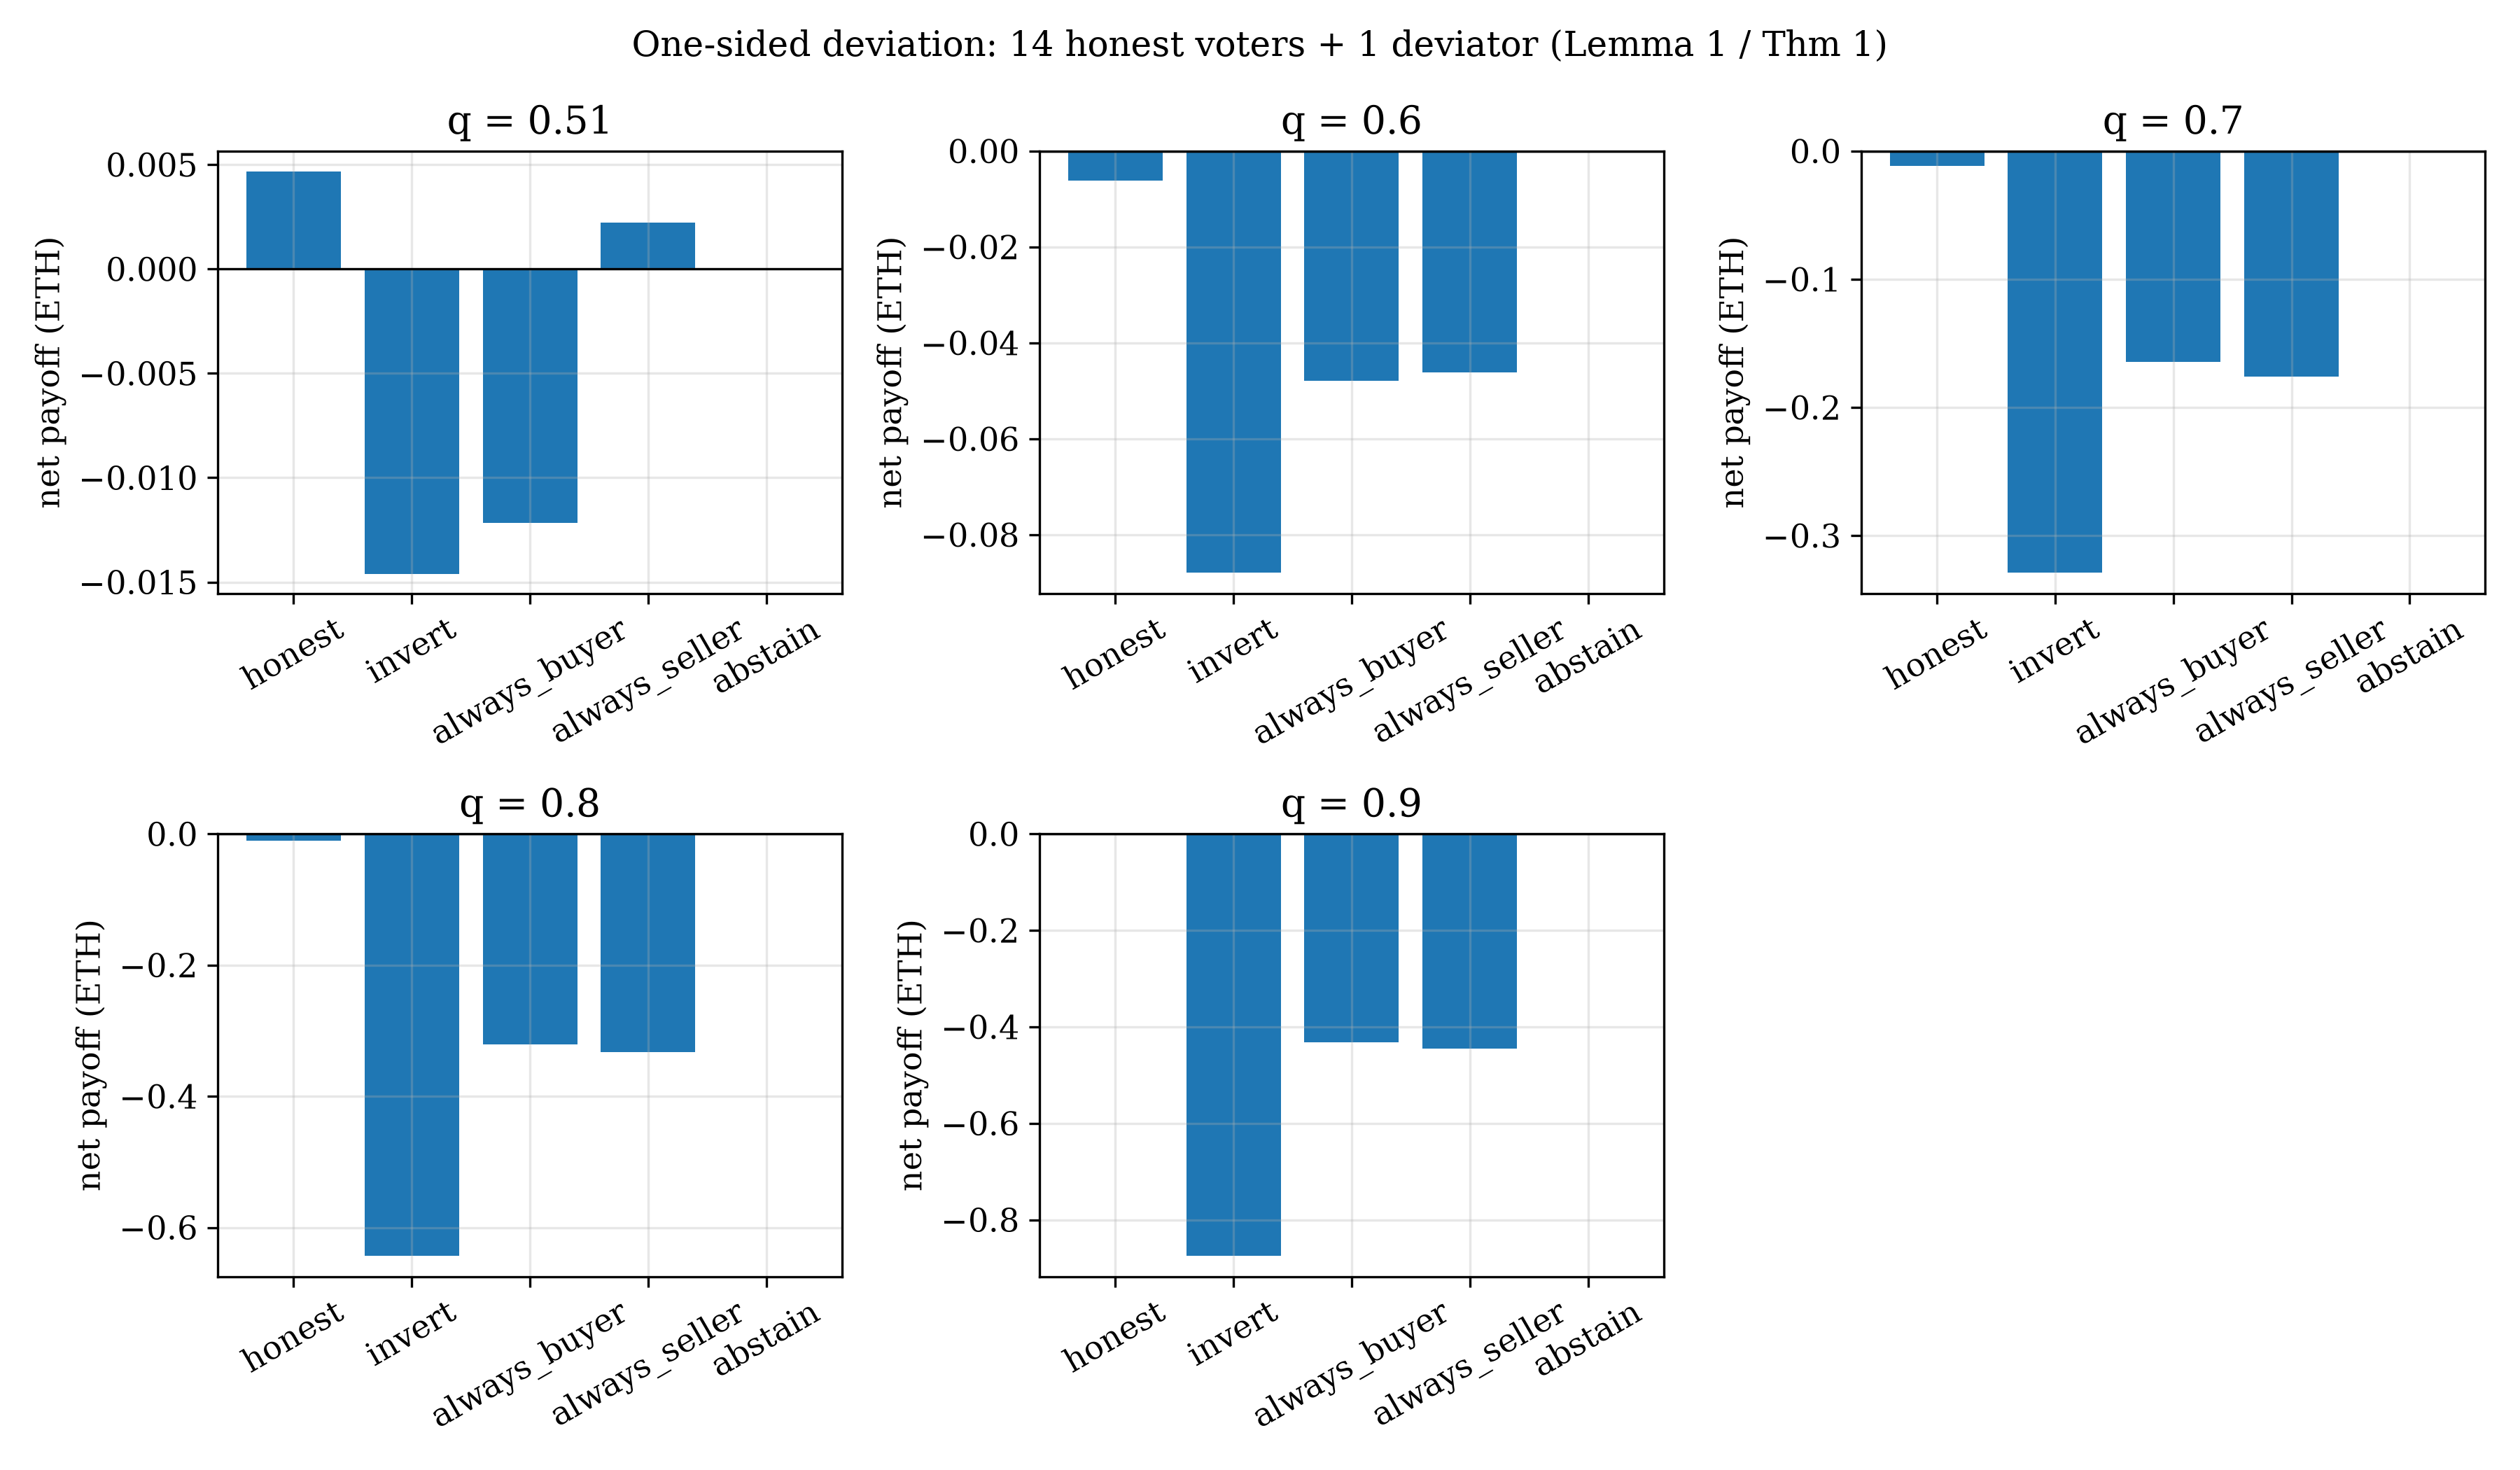
\includegraphics[width=0.9\linewidth]{exp1_honest_equilibrium.png}
\caption{Exp.\ 1 -- deviator mean net payoff vs.\ signal accuracy $q$. The gap
between the honest strategy and the invert/fixed strategies grows monotonically
with $q$, consistent with the bound
$p_{\sigma_{i}} - p_{\bar\sigma_{i}} \ge (2q - 1) - \varepsilon_{n}$ of
Lemma~\ref{lem:best-response}. (Figure: \texttt{simulation/plots/exp1\_honest\_equilibrium.png}.)}
\label{fig:exp1}
\end{figure}

The honest strategy strictly dominates \emph{invert} and both fixed-direction
strategies at every $q$, and the gap is monotone in $q$: it widens from
$\approx 0.020$ ETH at $q = 0.51$ to $\approx 0.87$ ETH at $q = 0.9$, tracking
$(2q - 1)$ as Lemma~\ref{lem:best-response} predicts. This confirms that a
rational voter who believes others vote their signals has no profitable
deviation to misreporting, and that the truthful profile of
Theorem~\ref{thm:incentive} is empirically sustained. The single-voter
estimator is noisy (the deviator's 95\% CI is roughly an order of magnitude
wider than the honest block's mean), so the honest deviator's point estimates
are statistically indistinguishable from the other honest voters' mean and from
zero.

\emph{Honest discussion.} The table also exposes an MVP limitation. The
abstention strategy yields exactly $0$ by construction (abstainers always
recover their stake), and the honest deviator's net converges to $\approx 0$
as $q \to 1$. A \emph{myopic} voter is therefore nearly indifferent between
honest voting and free abstention in single-period monetary terms: the
per-round honest bonus is small relative to the forfeiture risk. This is the
quantitative confirmation that the mechanism requires the \emph{multi-period}
reputation--guarantee pricing loop of Section~\ref{sec:pricing} to close the
incentive: in the full protocol, sustained participation in adjudication grows
a voter's reputation (lowering the guarantee premium on her own trades), while
abstainers are excluded from governance rewards -- the loop converts the
single-period tie into a strict multi-period dominance.

\subsubsection*{Exp.\ 2 -- Collusion resistance (Theorem~\ref{thm:collusion}).}

We fix $n = 21$ voters, the true state BUYER, signal accuracy $q = 0.85$, and
a collusion of $c$ adversarial voters who \emph{always} vote SELLER; the
remaining $21 - c$ voters are honest. We sweep $c/n$ and measure the
probability that the verdict is \emph{flipped} to the coalition's side over
$2000$ replications. Table~\ref{tab:exp2} and Figure~\ref{fig:exp2} report the
results.

\begin{table}[t]
\centering
\caption{Exp.\ 2 -- flip probability vs.\ coalition size, $n = 21$, true state
BUYER, $q = 0.85$, $2000$ replications,
\texttt{simulation/results/exp2\_collusion.csv}. The flip probability stays
below $1\%$ up to a $38\%$ coalition and jumps to certainty at
$14/21 = 2h$ (with $h = 7$ honest voters).}
\label{tab:exp2}
\small
\setlength{\tabcolsep}{5pt}
\begin{tabular}{lcccccc}
\hline
Colluders $c$ & $0, 2, 4$ & $6$ & $8$ & $10$ & $12$ & $14{+}$ \\
Coalition share & $\le 0.190$ & $0.286$ & $0.381$ & $0.476$ & $0.571$ & $\ge 0.667$ \\
Flip rate & $0.000$ & $0.0005$ & $0.0075$ & $0.079$ & $0.397$ & $1.000$ \\
\hline
\end{tabular}
\end{table}

\begin{figure}[t]
\centering
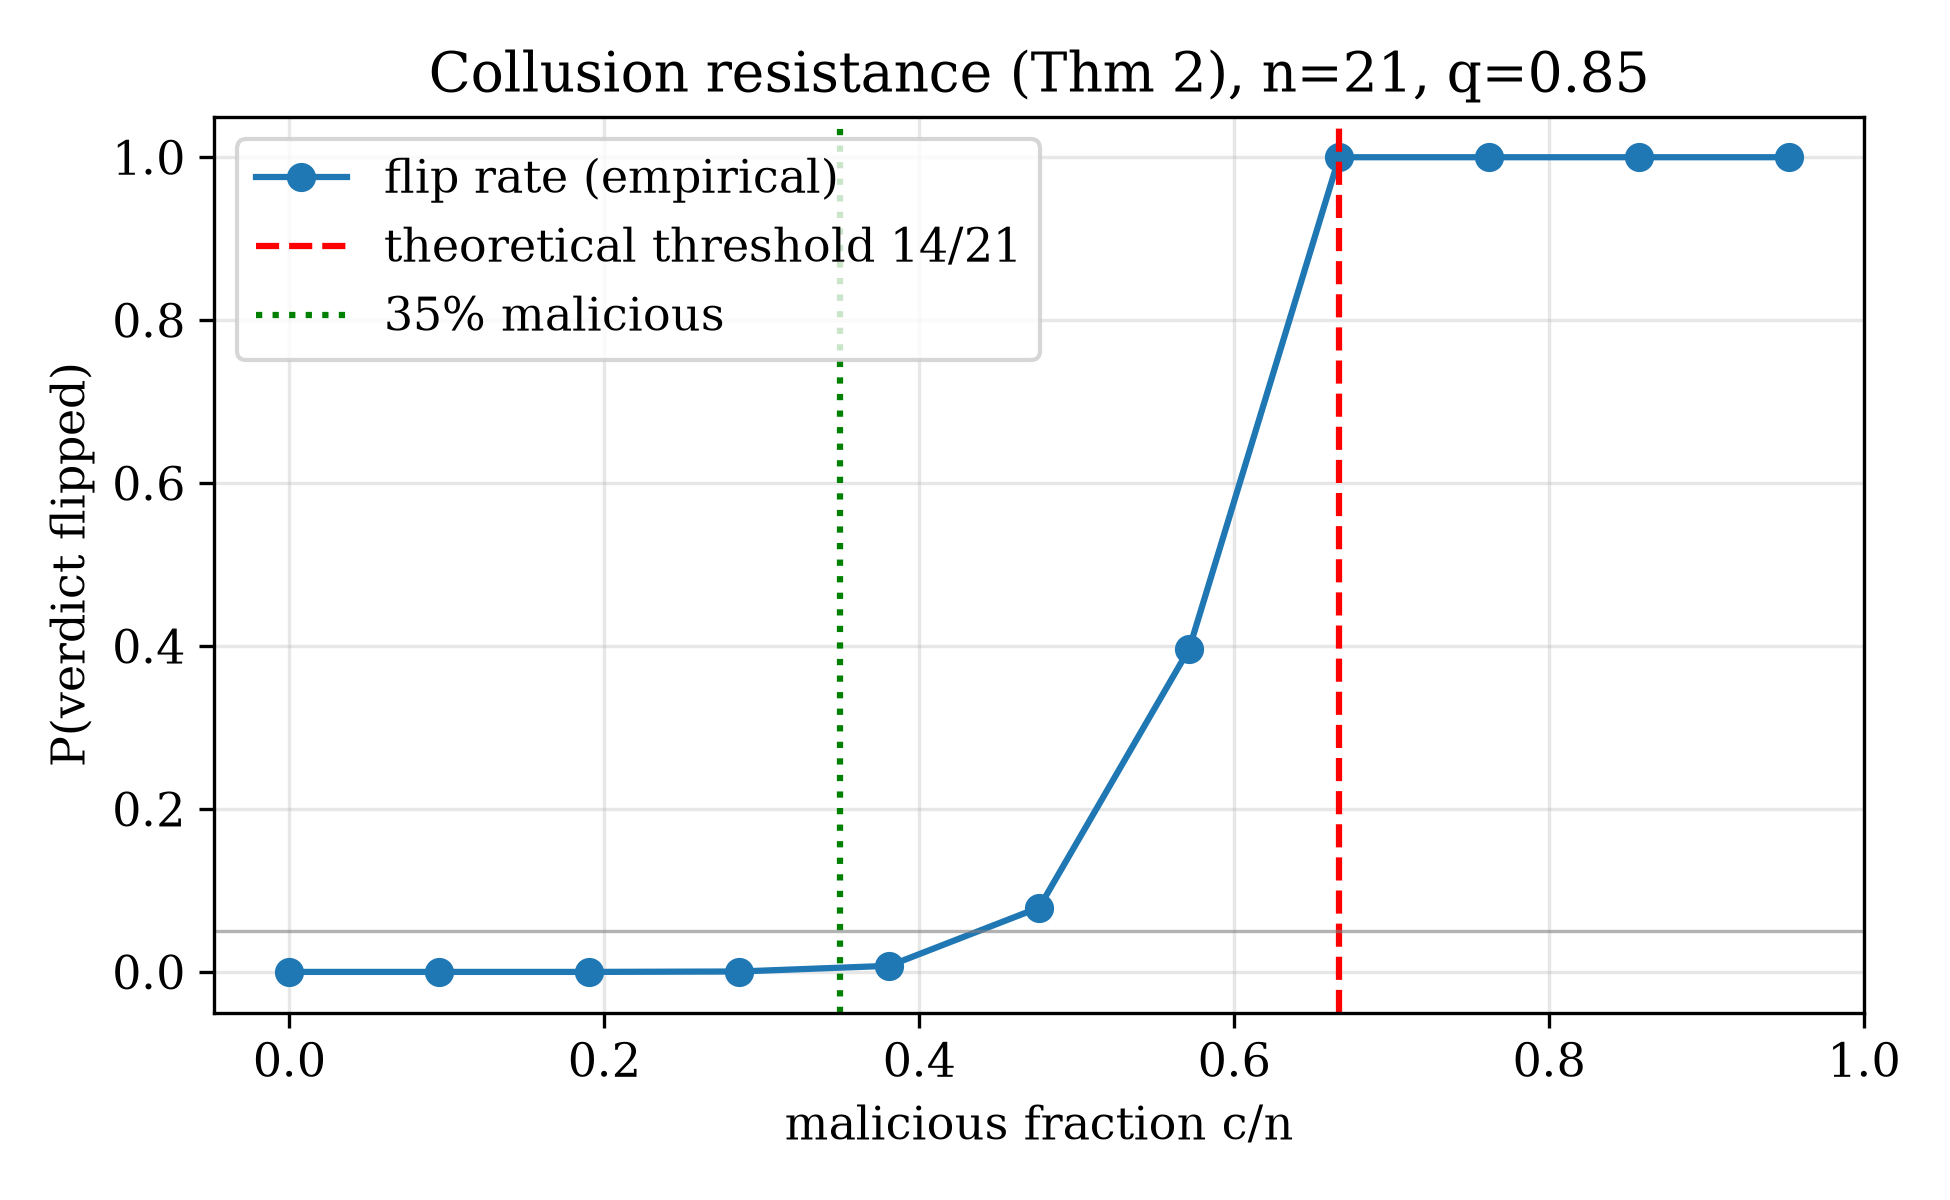
\includegraphics[width=0.9\linewidth]{exp2_collusion.png}
\caption{Exp.\ 2 -- flip probability as a function of the adversarial
coalition share. The curve is flat near zero up to a third of the electorate
and rises superlinearly to certainty at $2/3$. (Figure:
\texttt{simulation/plots/exp2\_collusion.png}.)}
\label{fig:exp2}
\end{figure}

A coalition of up to $38\%$ of the effective voters flips fewer than $1\%$ of
cases ($0.0075$ at $c/n = 0.381$), confirming the strategic-harmlessness claim
of Theorem~\ref{thm:collusion} (which guarantees it only up to $35\%$). The
flip probability then rises superlinearly -- $0.079$ at $c/n \approx 0.476$,
$0.397$ at $c/n \approx 0.571$ -- and becomes exactly $1$ at
$c/n = 2/3$ ($c = 14 = 2h$). Two observations sharpen the theory. First, the
empirical flip is a \emph{smooth} probability, not a step: the attacker
accumulates partial flip probability before the supermajority barrier. Second,
the theoretical sufficient bound $\lceil 13h/7 \rceil$ (with $h = 7$,
$\lceil 13 \rceil = 13$) is confirmed as a \emph{conservative} sufficient
condition under the $6500$-BPS approximation -- certainty is reached only at
the ideal two-thirds point $c = 14$. Below the barrier the coalition not only
fails to flip the verdict but, when it loses, forfeits its stakes to the
honest majority (Definition~\ref{def:settlement}).

\subsubsection*{Exp.\ 3 -- Sybil resistance (Theorem~\ref{thm:sybil}).}

We fix $h = 14$ honest voters and let an adversary create $k$ Sybil identities,
each costing $\texttt{registrationFee} = 0.1$ ETH plus a $1.0$-ETH vote stake
($1.1$ ETH per identity), all voting SELLER against the true state BUYER. We
sweep $k$ and measure both the flip probability and the total attack cost.
Table~\ref{tab:exp3} and Figure~\ref{fig:exp3} report the results.

\begin{table}[t]
\centering
\caption{Exp.\ 3 -- Sybil flip probability and total attack cost vs.\ number
of Sybil identities $k$ ($h = 14$ honest, fee $0.1$ + stake $1.0$ ETH per
identity), \texttt{simulation/results/exp3\_sybil.csv}.}
\label{tab:exp3}
\small
\setlength{\tabcolsep}{5pt}
\begin{tabular}{lcccccccc}
\hline
$k$ & $0{-}8$ & $10$ & $12$ & $16$ & $20$ & $22$ & $24$ & $26$ \\
Flip rate & $0.002$ & $0.013$ & $0.041$ & $0.147$ & $0.355$ & $0.648$ & $0.900$ & $1.000$ \\
Cost (ETH) & $\le 8.8$ & $11.0$ & $13.2$ & $17.6$ & $22.0$ & $24.2$ & $26.4$ & $28.6$ \\
\hline
\end{tabular}
\end{table}

\begin{figure}[t]
\centering
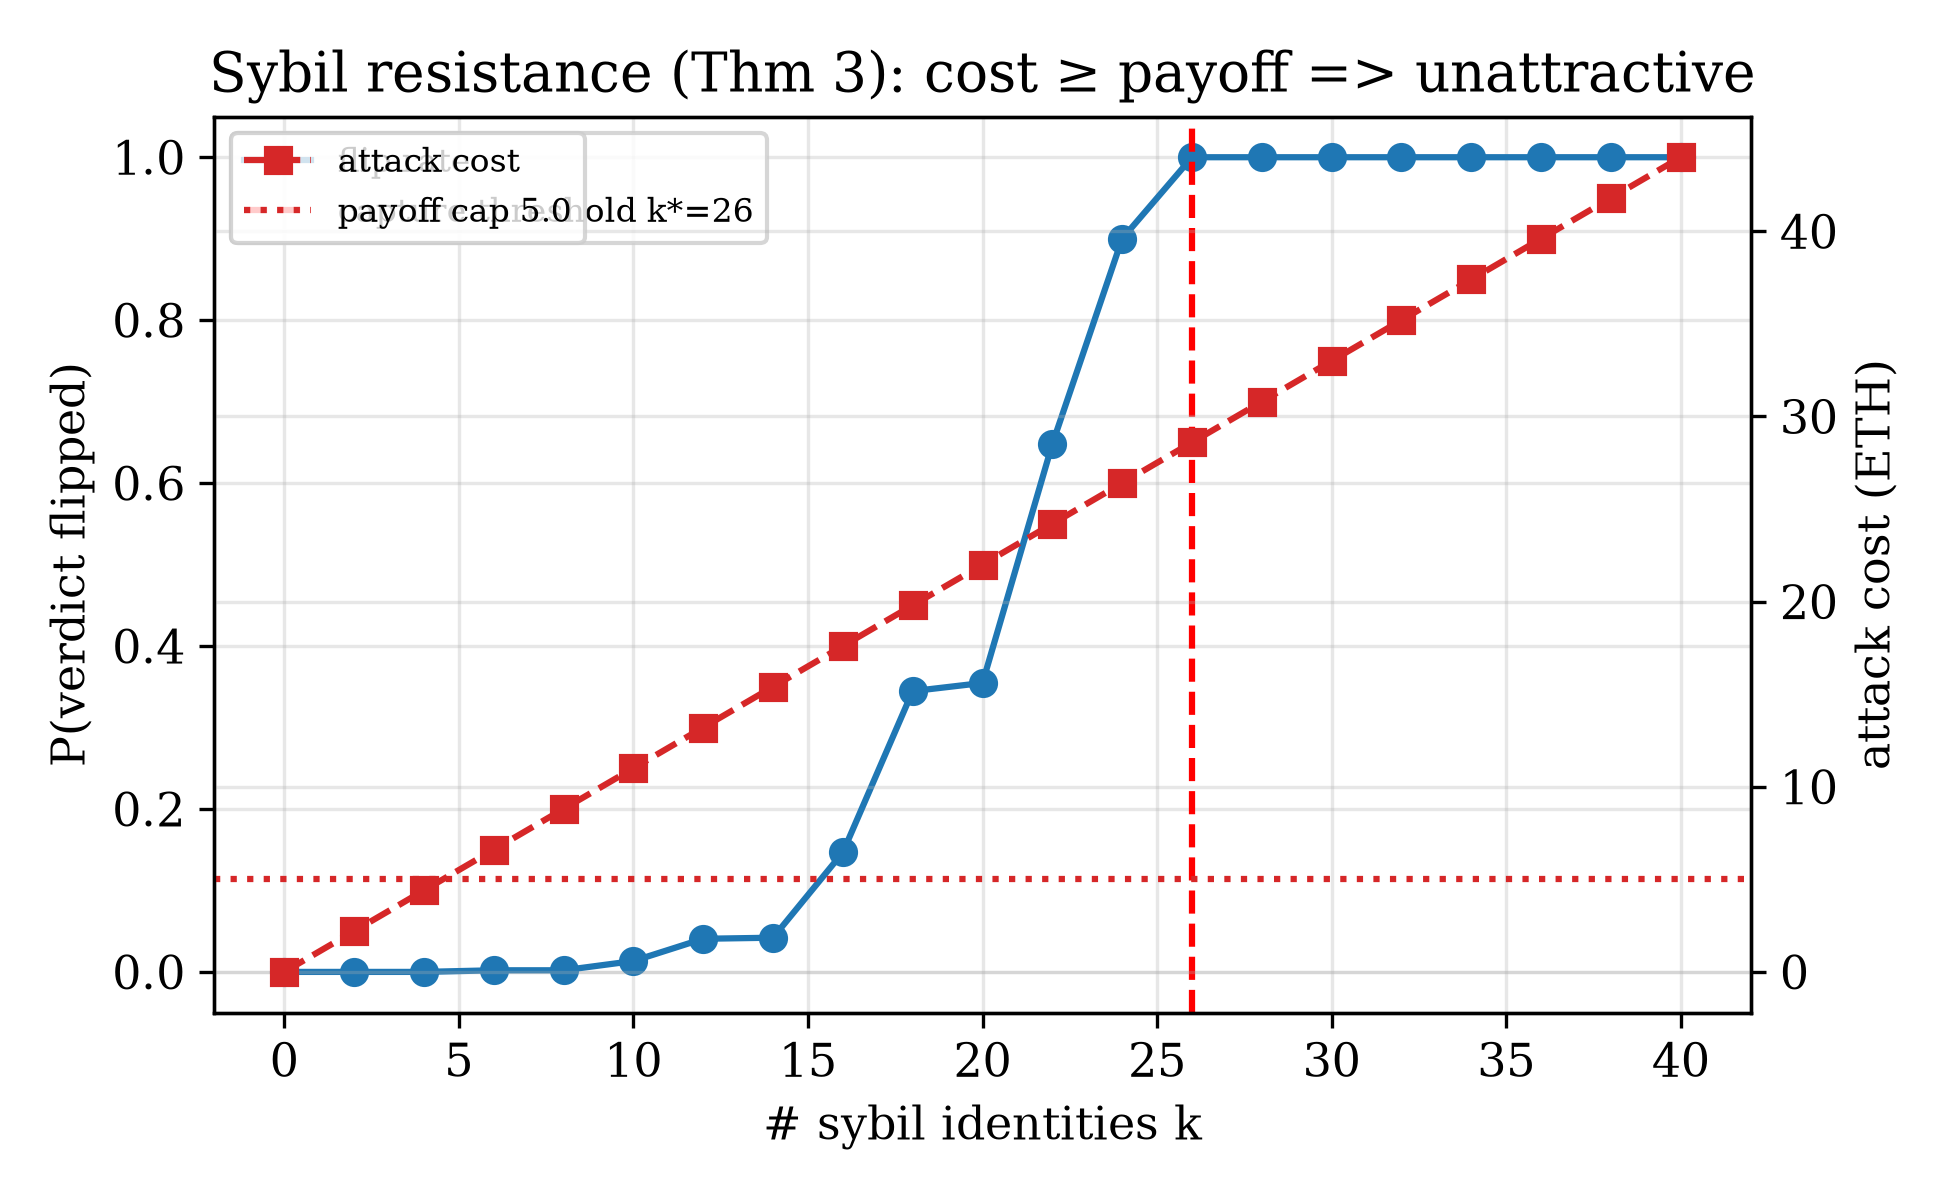
\includegraphics[width=0.9\linewidth]{exp3_sybil.png}
\caption{Exp.\ 3 -- Sybil flip probability and attack cost. High flip
probability requires $k \ge 22$ identities costing at least $24.2$ ETH, an order
of magnitude above any realistic dispute-value cap. (Figure:
\texttt{simulation/plots/exp3\_sybil.png}.)}
\label{fig:exp3}
\end{figure}

A flip probability of $0.648$ requires $k = 22$ identities at a cost of
$24.2$ ETH; it reaches $0.9$ at $k = 24$ ($26.4$ ETH) and certainty at
$k = 26$ ($28.6$ ETH). The theoretical sufficient bound of
Theorem~\ref{thm:sybil}, $\lceil 13h/7 \rceil = \lceil 13 \cdot 14/7 \rceil
= 26$, is again confirmed as a conservative upper bound (measured certainty at
$k = 26$). The realistic attack is cost-prohibitive: the maximum extractable
value of a captured verdict -- trade value plus premium -- is on the order of
$5$ ETH in the calibrated scenario, roughly a fifth of the $24.2$-ETH minimum
for a high-probability flip, so an expected-value-maximizing adversary does not
mount the attack. The observed critical point ($k \approx 22$) is slightly
below the pure theory because honest signal noise ($1 - q = 0.15$ here) gives
the attack side some free votes, exactly as Remark~\ref{rem:sybil-mvp} warns
for the capital-only barrier.

\subsubsection*{Exp.\ 4 -- Deterministic fund conservation (Lemma~\ref{lem:conservation}).}

We generate $4000$ random cases with $n \in [5, 30]$, $q \in [0.55, 0.95]$, and
random voter strategies, and verify the conservation identity of
Lemma~\ref{lem:conservation}: $\sum_{i} P_{i} = (m_{B} + m_{S} + m_{\bot})v -
\delta$ for effective cases and the full pool for void cases. The result is
exact: of the $4000$ cases, $1993$ settle effective and $2007$ void, and the
maximal absolute deviation of $\sum_{i} \text{net}_{i}$ from its expected value
is $0$ wei on \emph{every} path. Conservation holds exactly up to the bounded
dust term $\delta = (v \cdot m_{\ell}) \bmod m_{w}$ wei, which is the only value
left in the voting contract after settlement (data:
\texttt{simulation/results/exp4\_fund\_conservation.txt}). This is a direct,
whole-distribution confirmation of Lemma~\ref{lem:conservation} and
Table~\ref{tab:escrow-conservation}.

\subsubsection*{Exp.\ 5 -- Why a two-thirds supermajority
(Section~\ref{sec:threshold}).}

We fix $n = 15$ all-honest voters, $q = 0.7$, and scan
\texttt{MAJORITY\_BPS} over $\{5000, 5500, 6000, 6500, 7000\}$, measuring the
correct-verdict rate and the void rate over $3000$ replications. Table~\ref{tab:exp5}
and Figure~\ref{fig:exp5} report the results.

\begin{table}[t]
\centering
\caption{Exp.\ 5 -- threshold scan of \texttt{MAJORITY\_BPS}, $n = 15$,
all honest, $q = 0.7$, $3000$ replications,
\texttt{simulation/results/exp5\_threshold\_scan.csv}. At the deployed
$6500$ BPS the mechanism achieves a $0.721$ correct-verdict rate at a $0.275$
void rate.}
\label{tab:exp5}
\small
\setlength{\tabcolsep}{5pt}
\begin{tabular}{lccccc}
\hline
\texttt{MAJORITY\_BPS} & $5000$ & $5500$ & $6000$ & $6500$ & $7000$ \\
Correct rate & $0.947$ & $0.856$ & $0.856$ & $0.721$ & $0.512$ \\
Void rate & $0.000$ & $0.125$ & $0.125$ & $0.275$ & $0.487$ \\
\hline
\end{tabular}
\end{table}

\begin{figure}[t]
\centering
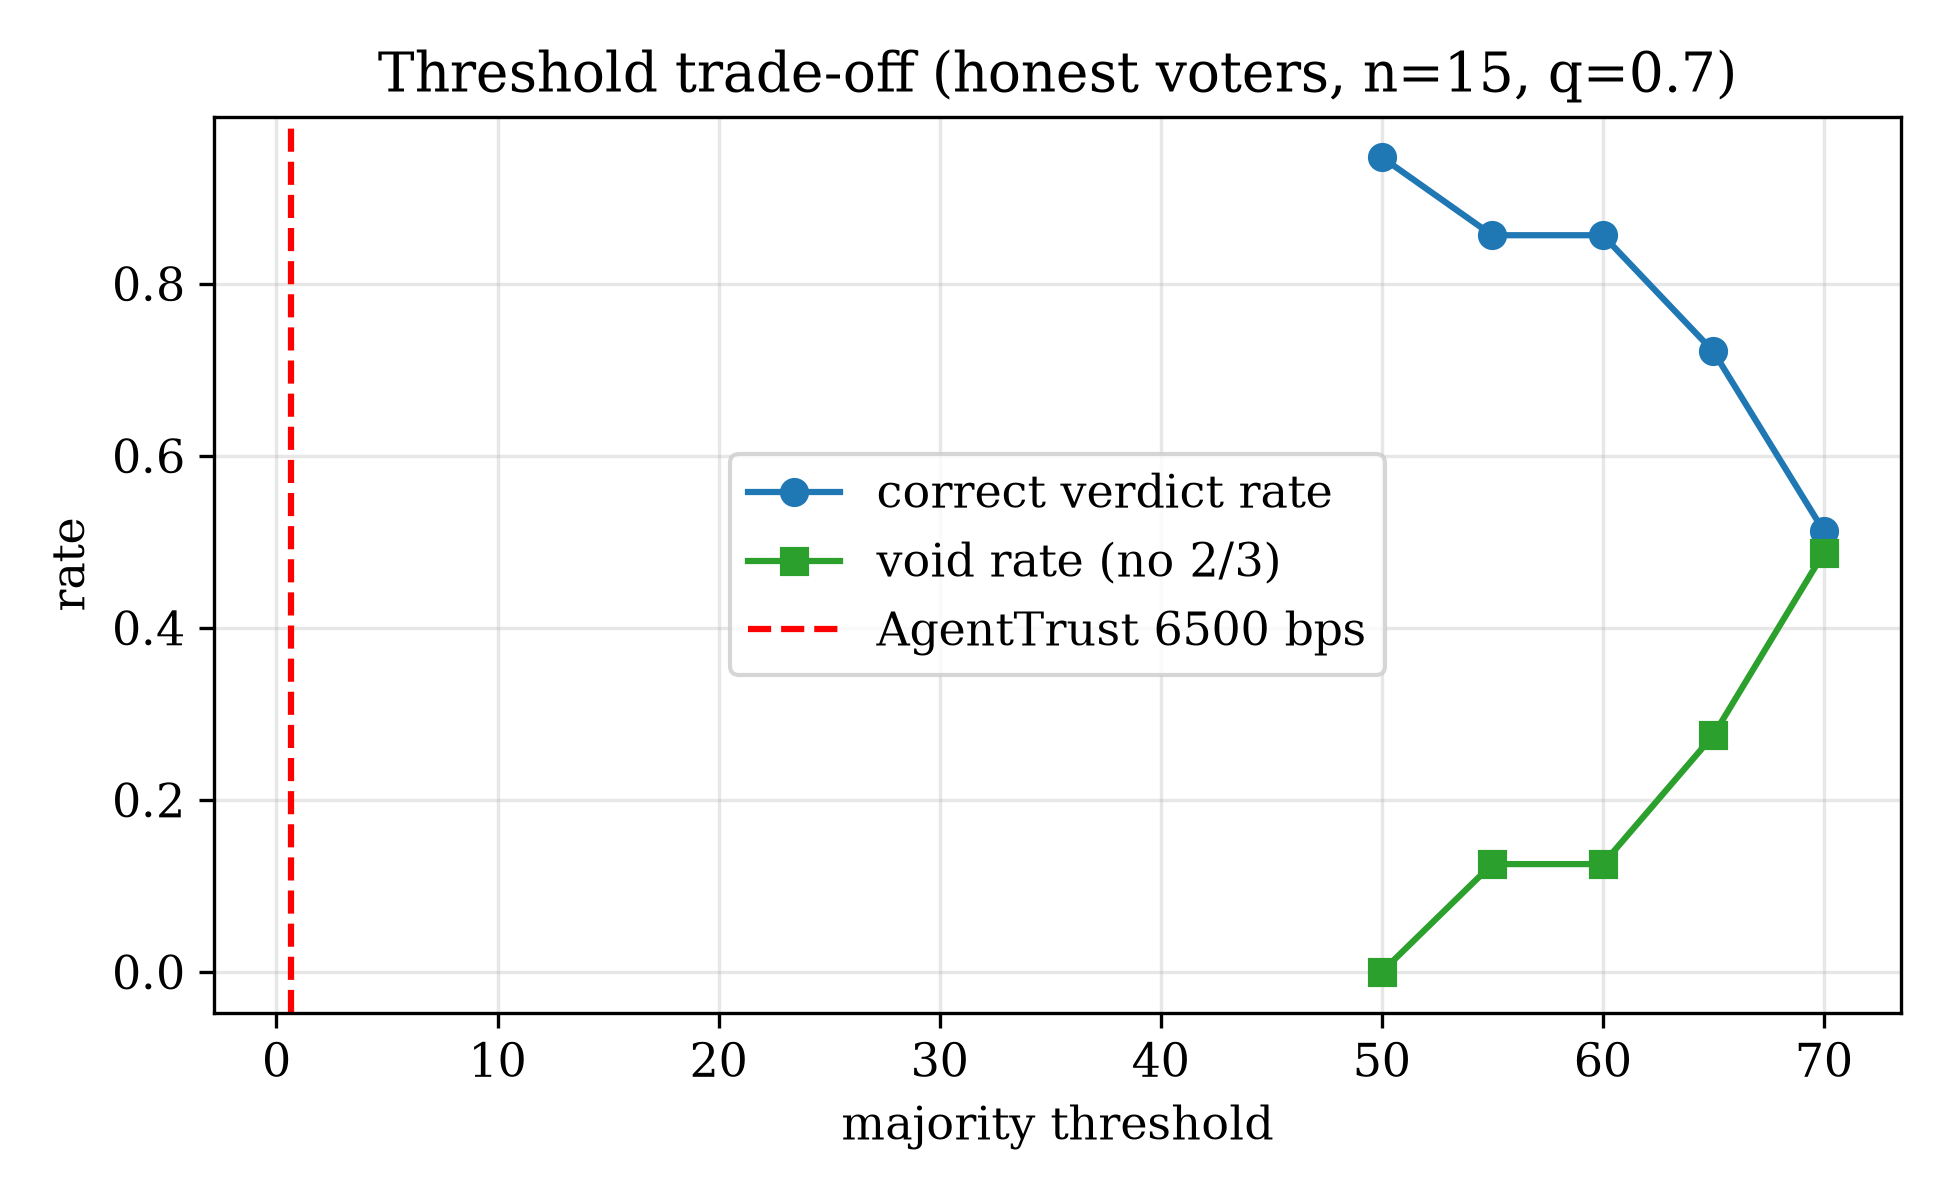
\includegraphics[width=0.9\linewidth]{exp5_threshold_scan.png}
\caption{Exp.\ 5 -- correct-verdict and void rates vs.\ \texttt{MAJORITY\_BPS}.
A lower threshold maximizes correctness but forfeits collusion resistance
(Exp.\ 2); the deployed $6500$ is the engineering compromise. (Figure:
\texttt{simulation/plots/exp5\_threshold\_scan.png}.)}
\label{fig:exp5}
\end{figure}

Lowering the threshold maximizes correctness ($0.947$ at $5000$ BPS, i.e.\ a
bare majority) but, as Exp.\ 2 showed, a $1/2$ threshold lets a one-third
coalition dictate outcomes. Raising it to $7000$ BPS voids nearly half of all
cases ($0.487$), because even small honest signal noise and abstention deny the
supermajority. The deployed $6500$ BPS sits at the engineering compromise:
$0.721$ correctness at a $0.275$ void rate, tolerating a coordinated malicious
minority of up to a third (Theorem~\ref{thm:collusion}) while keeping
legitimate cases alive -- a direct empirical restatement of the three
arguments in Section~\ref{sec:threshold}.

\paragraph{Summary of limitations.}
Four limitations of the current prototype are documented and left to future
work. (i) \emph{Free abstention}: Exp.\ 1 shows single-period honest net
$\approx$ abstention net $= 0$, so the incentive closes only through the
multi-period reputation loop of Section~\ref{sec:pricing}; the MVP contracts do
not yet penalize or reward participation directly. (ii) \emph{Dust}: the
bounded integer remainder $\delta < m_{w}$ wei stays in the voting contract;
Exp.\ 4 confirms it is the only unconserved value, and a batched-settlement
refinement removes it. (iii) \emph{Engineering threshold}: $6500/10000$ is an
approximation of $2/3$ that marginally lowers the adversarial requirement
(factor $13/7 \approx 1.857$ instead of $2$) at negligible security cost.
(iv) \emph{Demo-grade chain}: the canonical deployment is a local Anvil chain
for demonstration and the Base Sepolia testnet for integration; the MVP is not
mainnet-deployed. Additional MVP simplifications noted in the code are the
owner-only \texttt{openCase} (the full design drives case opening from the
escrow), the absence of a dispute window, claim-based (non-Merkle) settlement,
and no ZK-based random jury sampling.

% ============================================================================
\subsection{Deployment}
\label{sec:deploy}
% ============================================================================

\paragraph{Local demonstration chain.}
The canonical deployment runs on a local Anvil node
(\texttt{anvil --chain-id 31337 --port 8545}). The deploy script
\texttt{contracts/script/Deploy.s.sol} executes in the fixed order
\textsf{AgentRegistry} $\to$ \textsf{ReputationHub} $\to$
\textsf{GuaranteeEscrow} $\to$ \textsf{SchellingVoting}, then performs the two
linkage steps required by the architecture: it authorizes the escrow and the
voting contract as \textsf{ReputationHub} writers
(\texttt{setAuthorizedCaller}) and transfers escrow ownership to the voting
contract (\texttt{transferOwnership}), so that a community verdict can drive
settlement. Anvil's deterministic address derivation yields stable addresses
that are pre-filled into \texttt{frontend/lib/config.ts}
(Table~\ref{tab:addresses}); re-deploying does not change them. With the
default \texttt{registrationFee = 0}, agents register for free, and the
three deterministic Anvil test accounts (each funded with $10000$ ETH) serve as
the seller, buyer, and guarantor/voter wallets of the five-minute
demonstration in \texttt{contracts/demo/DEMO.md}.

\begin{table}[t]
\centering
\caption{Deterministic deployment addresses on the local Anvil chain
(chain id $31337$), as produced by
\texttt{forge script script/Deploy.s.sol --broadcast} and wired into
\texttt{frontend/lib/config.ts}.}
\label{tab:addresses}
\small
\setlength{\tabcolsep}{4pt}
\begin{tabular}{ll}
\hline
Contract & Anvil address \\
\hline
\textsf{AgentRegistry} & \texttt{0x5fBDB2315678afecb367f032d93F642f64180aa3} \\
\textsf{ReputationHub} & \texttt{0xe7f1725E7734CE288F8367e1Bb143E90bb3F0512} \\
\textsf{GuaranteeEscrow} & \texttt{0x9fE46736679d2D9a65F0992F2272dE9f3c7fa6e0} \\
\textsf{SchellingVoting} & \texttt{0xCf7Ed3AccA5a467e9e704C703E8D87F634fB0Fc9} \\
\hline
\end{tabular}
\end{table}

\paragraph{Testnet deployment (Base Sepolia).}
To move to a public testnet the operator runs the same script against
\texttt{https://sepolia.base.org} with verification enabled:
\begin{verbatim}
forge script script/Deploy.s.sol --rpc-url https://sepolia.base.org \
  --broadcast --verify --private-key "$PRIVATE_KEY"
\end{verbatim}
The pre-requisites are: a testnet private key (loaded via
\texttt{vm.envUint("PRIVATE\_KEY")}, never committed to the repository),
test ETH obtained from a Base Sepolia faucet for the deployer and the demo
wallets, and block-explorer API access for source verification. After
deployment the four addresses are written into
\texttt{frontend/lib/config.ts} and \texttt{wagmi} is pointed at
\texttt{baseSepolia} (which is exactly what \texttt{NEXT\_PUBLIC\_CHAIN =
base-sepolia} selects at build time).

\paragraph{Static front-end hosting.}
Because the front end is statically exported, it is deployed to GitHub Pages.
The workflow (\texttt{.github/workflows/deploy-pages.yml}) builds the
application with \texttt{NEXT\_PUBLIC\_CHAIN=base-sepolia} and
\texttt{NEXT\_PUBLIC\_BASE\_PATH=/<repository-name>} (e.g.\
\texttt{/multiagent/}) on every push to \texttt{main}, uploads the
\texttt{frontend/out} artifact, and publishes it. The same containerized path
is available via \texttt{docker compose}, which starts the Anvil node, runs
the deploy script, and serves the front end with one command.

% ============================================================================
%  End of Chapter 5 (paper/implementation.tex). Numbering continues Chapter 4
%  (paper/mech-design.tex); no new theorem/lemma/proposition/corollary
%  environments are introduced in this chapter.
% ============================================================================

% ============================================================================
%  Chapter 6: Conclusion
% ============================================================================
\section{Conclusion}
\label{sec:conclusion}

We presented a decentralized guarantee and arbitration layer for agent-to-agent commerce built on
the Schelling-point reputation community: registered agent identities, a guaranteed escrow,
staked-voting adjudication, and reputation-driven guarantee pricing, closed into one on-chain loop.
We proved that under a two-thirds supermajority rule honest voting is incentive compatible, that a
coordinated malicious minority of at most $35\%$ of voters is strategically harmless, that Sybil
attacks are unprofitable because adversarial voting power scales linearly in expenditure, and that
the mechanism conserves funds exactly. We instantiated the protocol in Solidity with 38 passing
tests and an end-to-end demo, and validated the theory by Monte-Carlo simulation built on
\textsf{mesa}. To our knowledge this is the first protocol to tie adjudication, guarantees, and
reputation into a single verifiable cycle, addressing the accountability vacuum of anonymous
machine-to-machine commerce (Q2) with an economically self-sustaining governance mechanism (Q3).

\paragraph{Limitations.}
The current MVP makes several deliberate simplifications, each flagged on-chain and in the theory:
(i) \emph{free abstention} --- abstainers are refunded rather than penalized, so the one-shot
monetary payoff of honest voting is only marginally better than abstaining; the reputational
tie-breaker of the closed loop is therefore load-bearing for participation (Section~\ref{sec:pricing});
(ii) \emph{integer dust} --- the majority reward's division remainder is stranded in the contract;
(iii) \emph{engineering threshold} --- $\texttt{MAJORITY\_BPS} = 6500$ approximates two-thirds with
integer-safe arithmetic; (iv) \emph{demonstration chain} --- the deployment targets a local anvil
chain and, as a next step, a public testnet (Section~\ref{sec:deploy}); and (v) \emph{no random jury
selection} --- anyone can vote on any case, which the full design refines with ZK-augmented random
selection.

\paragraph{Future work.}
Short-term directions are: batch settlement to eliminate dust; the full identity barrier that binds
every vote to a registered, fee-paid agent ID; ZK-augmented random jury selection with privacy
adjustability; and a larger simulation study of threshold tuning, collusion dynamics, and
reputation-strategy equilibria. Longer term, the mechanism is designed to operate on a public
Ethereum L2 (Base) and to integrate with the ERC-8004 trustless-agent ecosystem; a production
deployment will follow the testnet checklist of Section~\ref{sec:deploy}. Compliance-wise, the
MVP uses testnet tokens with no real value; any tokenization would require an overseas-compliant
issuance structure, while liability remains anchored to real principals via the registry.

\paragraph{Concluding remark.}
The core design bet of this paper is that in an economy of autonomous agents, trust should be
\emph{earned, verified, and priced} --- not assumed. By making the community that arbitrates a
dispute the same community whose reputational and financial stakes depend on the verdict, the
Schelling-point reputation community turns truthful adjudication into the rational choice, and
turns reputation into a storable, revenue-bearing asset that prices the very guarantees that make
future agent-to-agent commerce safe.


\bibliographystyle{unsrt}
\bibliography{references}

\end{document}
